\documentclass{nihgrant}
\usepackage[utf8]{inputenc}

\usepackage{lipsum} % For dummy text

\title{NIH application}
\author{Geoffrey Brookshire}
\date{}

\begin{document}

\section*{Overview}

The \verb|nihgrant.cls| class provides a simple template for writing NIH grants. The format was current as of April 2019. This template is designed to maximize clarity, and to minimize space. When those two criteria conflict, I went with the choice that maximizes clarity.

\subsection*{Usage.}
Use \verb|\section*{}| for page headers, and use \verb|\subsection*{}| and \verb|\subsubsection*{}| for section names in the text. For references, I altered the \verb|abbrvnat.bst| style to write the last name first in the bibliography. The \verb|wrapfigure| environment is a good way to show figures without wasted space.

\subsection*{Example.}
On the next page, there's an example of what a Research Strategy section might look like.

\pagebreak

\section*{Significance}

\subsection*{Examples of references.} In an NIH grant, you want to communicate your novel hypotheses \cite{kuhn1962} in the context of information \cite{shannon1948} about prior studies.

\subsection*{Why do we always use Lorem Ipsum for dummy text?}
\lipsum[1-1]

\subsection*{It's pretendo Latin.} 
\lipsum[3-3]

% Example figure
\begin{wrapfigure}{r}{0.425\textwidth}
  \vspace{-0.25cm} % Mess with the spacing parameters to squeeze things in
  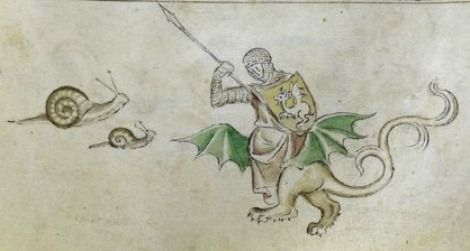
\includegraphics[scale=0.48]{Knight-fighting-snail-470.jpg}
%   \vspace{-0.5cm}
  \caption{
  \textbf{Example figure.}
  Here's a medieval drawing of a knight fighting snails.
}
\label{fig:example}
\vspace{-0.25cm}
\end{wrapfigure}

\subsubsection*{Isn't that bizarre?}
\lipsum[3-3]

\subsubsection*{You'd think it'd be easier to use a real text.}
\lipsum[4-4]

\section*{Approach}
\lipsum[5-5]

\pagebreak
\bibliography{bib} 

\end{document}
